\documentclass{article}

\usepackage{graphicx}
\usepackage{indentfirst}
\usepackage{enumitem}
\usepackage{geometry}
\usepackage{booktabs}
\usepackage{caption}
\usepackage{array}
\geometry{left=3cm, right=3cm, top=2cm, bottom=2cm}
\usepackage[colorlinks,linkcolor=blue]{hyperref}
\setlength{\parindent}{4em}

\title{\textbf{Software Requirements Specification} \\ {\textbf{Command-line-based Monopoly Game}}\\ {\large PolyU COMP3211 Software Engineering Project, Fall 2024}}
\author{\large Group 24}
\date{\today}

\begin{document}

\maketitle{}

\tableofcontents

\section{Preface}

This Software Requirements Specification (SRS) document is intended to provide a detailed overview of requirements of the development of Command-line-based Monopoly Game for our development team. 
It outlines the functional and non-functional requirements for each system requirement well-defined for basic user requirements of the software, as well as the constraints and assumptions that the development team should consider.

This is the second version of the SRS document, which is based on the feedback from the first version of the SRS document. More measurement metrics and description of system requirements are added to the document.

\section{Introduction}

The Command-line-based Monopoly Game (CMG) is expected to be a software system with command-line based user interface that simulates user experience and operation mechanisms of the classical Monopoly board game.
Meanwhile, CMG will provide features that allows portable saving of games in progress and customizing the game board with flexibility, in addition to the physical board game. 

CMG will provides system functions of starting a new game, loading a saved game, saving a game, customizing game boards, loading a customized game board, and playing the game
on the custom game board. In the game, the system will provide identical game rules as the classical Monopoly game, including the rules of moving the player token, buying properties, paying rent, drawing chance cards, declaring the winner, and so on.
For game board designers, the system will be implemented with a feature that allows them to customize the game board by adjusting the properties on an existing or a saved game board.

The system aims to provide a user-friendly interface design for users to interact with the system, and to provide a robust and reliable system that can handle various user behaviors and system exceptions.
By implementing the system with the Java programming language, the system will be able to run on any platform that supports Java Virtual Machine to reach the portability and compatibility goals.

\section{Glossary}

\paragraph{CMG} The Command-line-based Monopoly Game, which refers to this software system that simulates the classical Monopoly board game with command-line based user interface with additional features.
It consists of two main sections: the gaming procedures and the game board design procedures.

\paragraph{The Gaming Procedures and the Game Board Design Procedures} The two main sections of the CMG system. The gaming procedures are the procedures that are used to play the game, while the game board design procedures are the procedures that are used to design the game board.
Users are asked to choose which section they want to enter when they start the CMG system. Then they will be recognized as either a player or a game board designer.

\paragraph{Player} The user who plays the game in the CMG gaming procedures.

\paragraph{On Going Player and Bankrupt} Ongoing player is a player who is still in the game and has not been bankrupted. A player will be bankrupted if the player's cash is less than 0 after paying the rent or the penalty.
If a player is bankrupted, the player will be removed from the on going players, and the player's properties will be released to the game again. The bankrupted player can no longer do any operations.

\paragraph{Game Board Designer} The user who designs the game board in the CMG game board design procedures.

\paragraph{Game Board} The game board is an instance in CMG, which is viewed as a 2D grid that represents the game board of the classical Monopoly game. 
A game board can be only constructed by a Game Board File.

\paragraph{Game Board File} The file that stores the game board information in the CMG system. It can be loaded to the gaming procedures to construct a game board, and saved by or loaded to game board design procedures to be viewed in the instance of a game board.
Such files are expected to be in a specific format, e.g., .csv files or specialized .txt files, that can be recognized by a certain system routine, and located in a fixed relational location
for the ease of operations from source code.

\paragraph{Game in Progress} The game instance that is currently being played by the players in the CMG gaming procedures. A game will end when only one player who is not bankrupted is left, or the total number of rounds reaches 100.

\paragraph{Saved Game} The game instance that is saved by a player insides whether a game in progress or an ended game. 
A saved game can be reinitialized to continue as a game in progress or just to show the eventual status if the game instance reconstructed has ended.

\paragraph{Game Save (Game Save Files)} The file that store the game information for reconstruct a saved game instance. 
Such files are also expected to be in a specific format for ease of loading and saving, and located in a fixed relational location to the source code files.

\paragraph{Rounds and Turns} A round consists of multiple turns, and a turn consists of operations of a particular player.
A player can do multiple operations in a turn, such as querying the other players' information, printing the game board, saving the game, and so on.
A player's turn will once end automatically after the player rolls the dice and then moves to a new position.
The number of turns of a rounds is equal to the number of ongoing players in the game.

\paragraph{Properties} Properties are instances that is viewed as the grids on the game board. Properties are classified into two types: normal properties that can be bought, and the special properties that can effect the player's status in the game.
The special properties include GO, Income Tax, Chance, Jail Visiting, Go to Jail and Free Parking.

\paragraph{Property Price and Rent} If a normal property is not owned by any player, the player can buy the property with the price of the property if the player is currently on the property. If a player owns a property, the player can charge the rent to the other players who land on the property.

\paragraph{GO} The starting point of each player at the beginning of the gaming procedures. After that, a salary of HKD1500 will be given to every player each time they pass through.

\paragraph{Income Tax} The property that will charge the player 10\% of her money (rounded down to a multiple of 10) when the player lands on this property.

\paragraph{Chance} The property that will trigger a random change on player's money when the player lands on this property. 
The change is a multiple of 10 from -200 to 300.

\paragraph{Jail Visiting} The property that will not effect the player's status when the player lands on the Jail property.

\paragraph{Go to Jail} The property that will send the player to the Jail property when the player lands on this property. 

\paragraph{Jailing} The status of a player when she lands on the property Go to Jail. 
A player in jail can exit by accomplishing one of the following within her next three turns: rolling identical numbers on both dice (doubles), resulting in an immediate advancement by the number of spaces indicated by the double roll, or choosing to pay a fee of HKD 150 before rolling the dice on her subsequent two turns. 
Failing to roll doubles within the three turns mandates a payment of HKD 150. Upon payment of the fee, the player is released from jail and promptly moves the designated number of spaces determined by her subsequent dice roll.

\paragraph{Free Parking} The property that will not effect the player's status when the player lands on this property.


\section{User Requirements Definition}

\subsection{Player Use Cases}
The following use cases are defined for the player in the CMG system.
\begin{figure}[htbp]
    \centering
    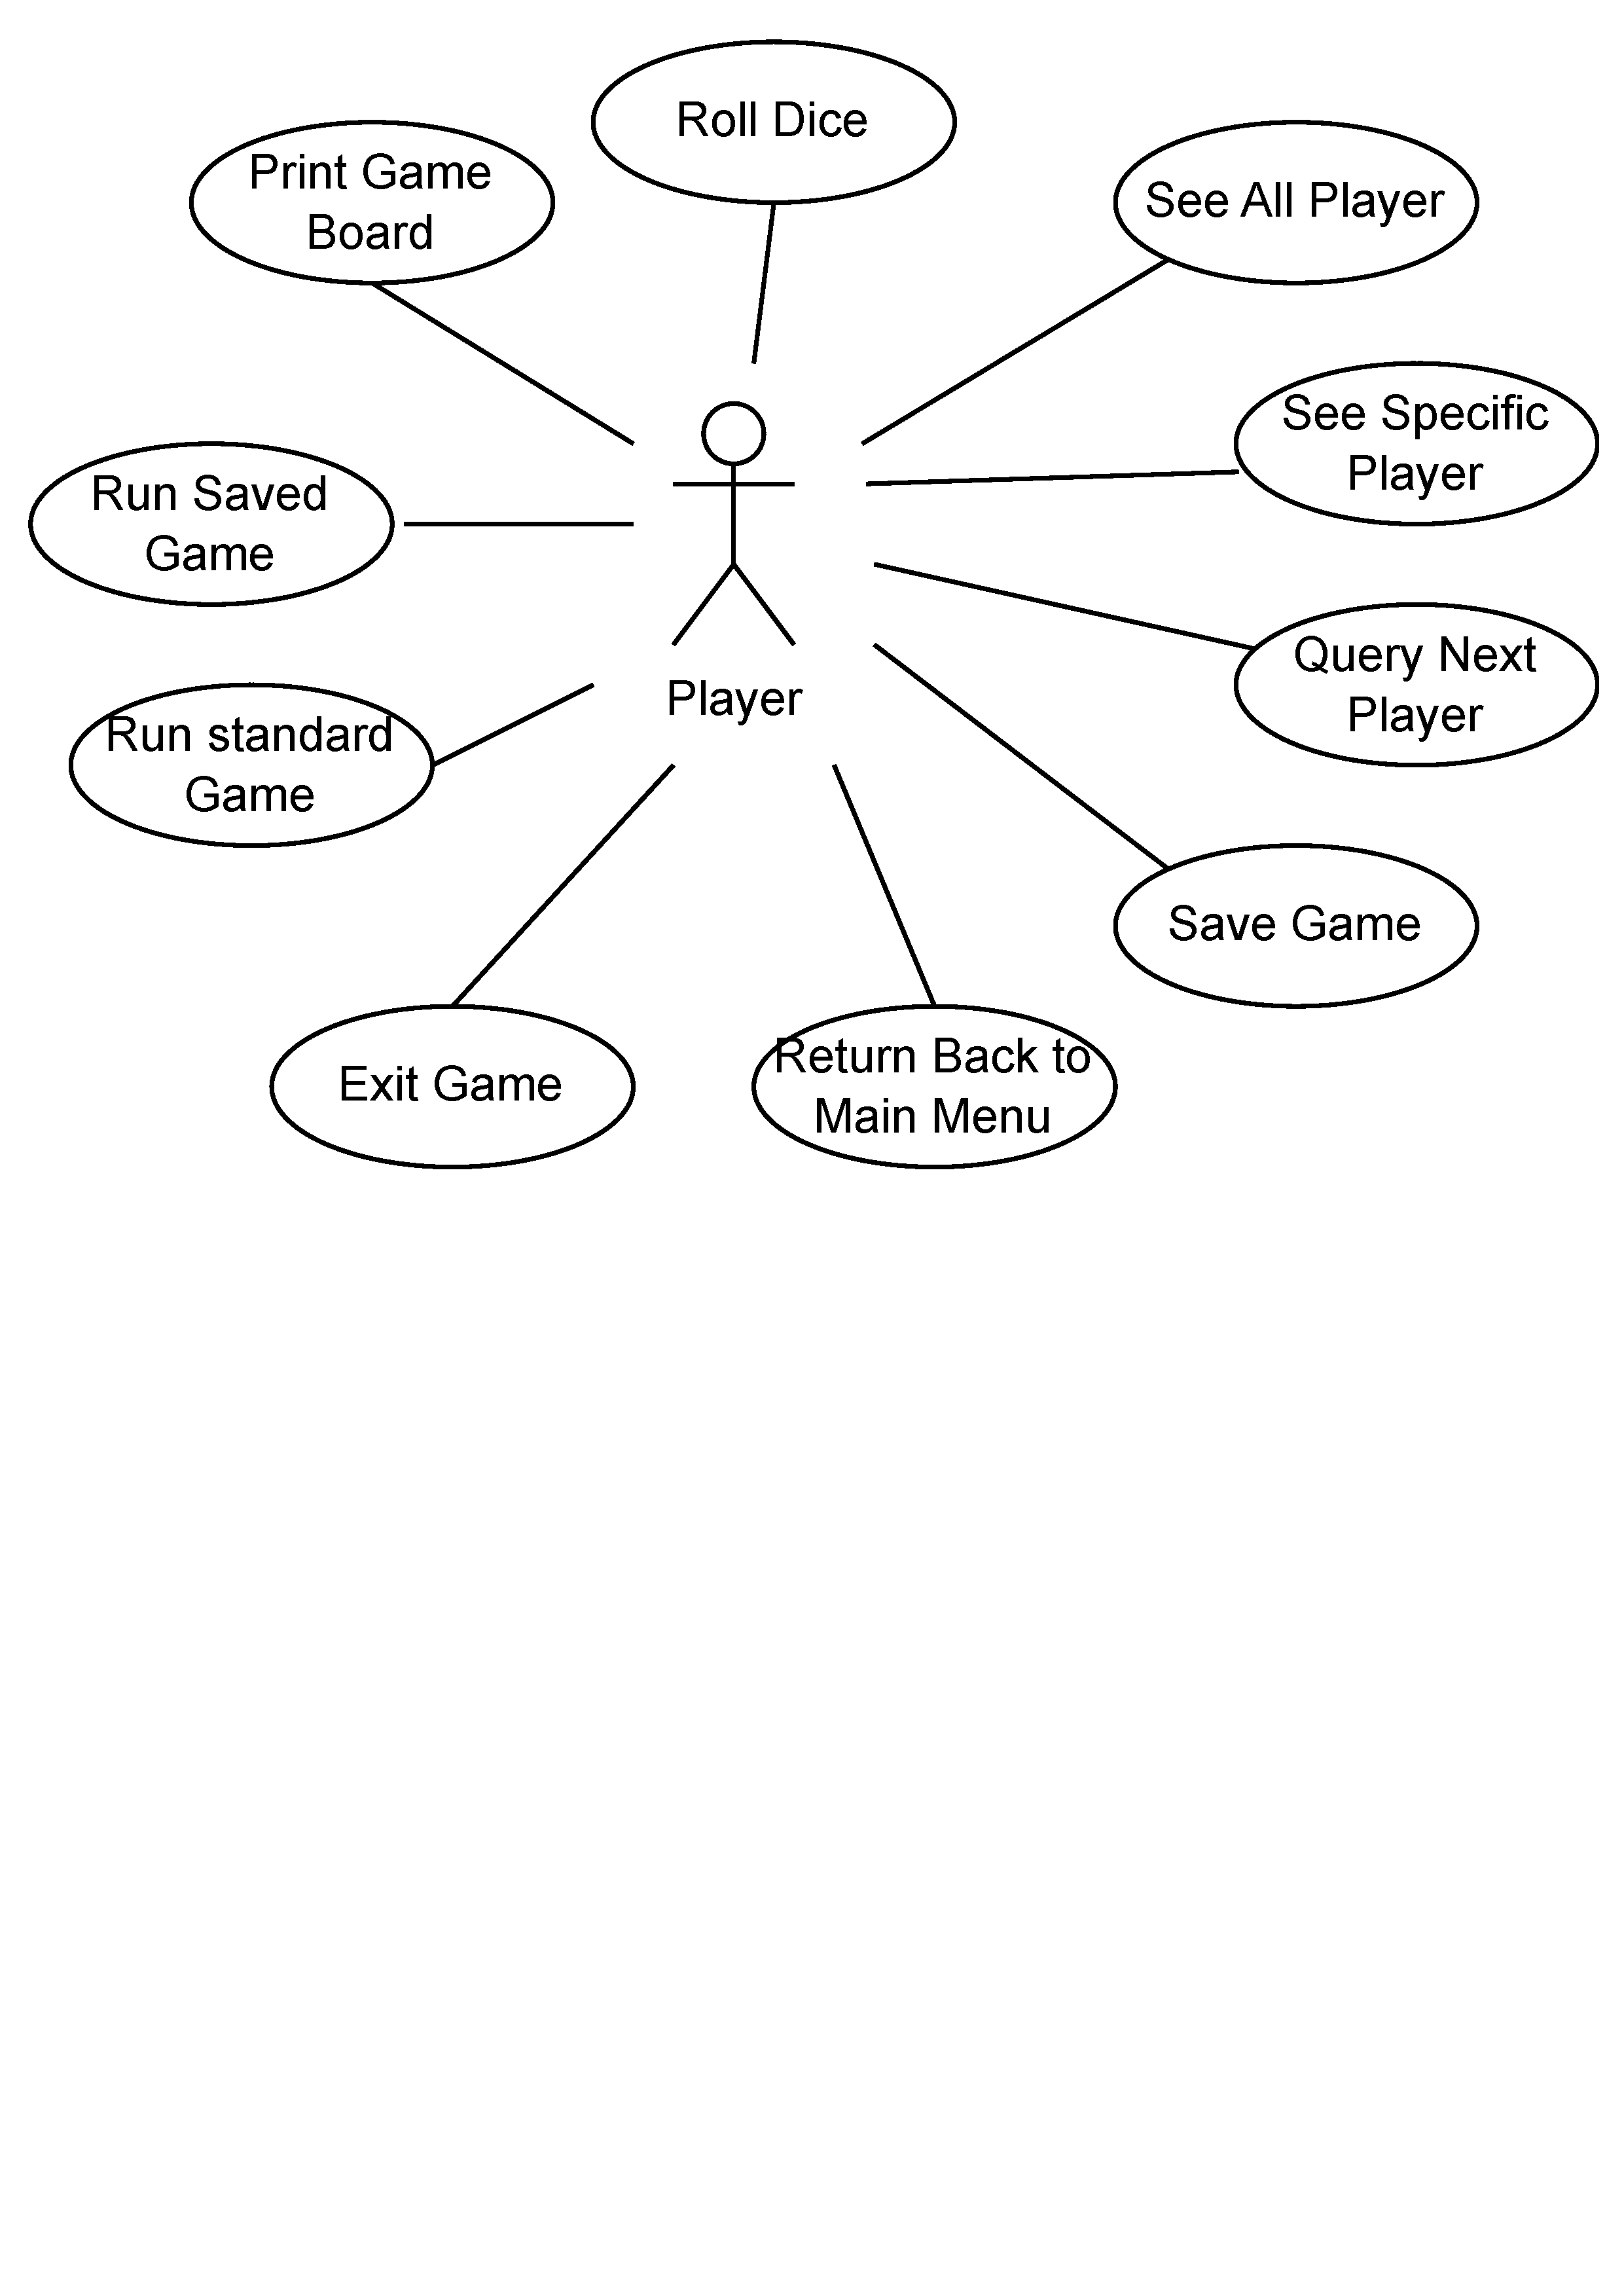
\includegraphics[width=0.6\textwidth]{crop_PlayerUseCase.drawio.pdf}
    \caption{Player Use Cases}
\end{figure}

\subsection{Game Board Designer Use Cases}
The following use cases are defined for the game board designer in the CMG system.
\begin{figure}[htbp]
    \centering
    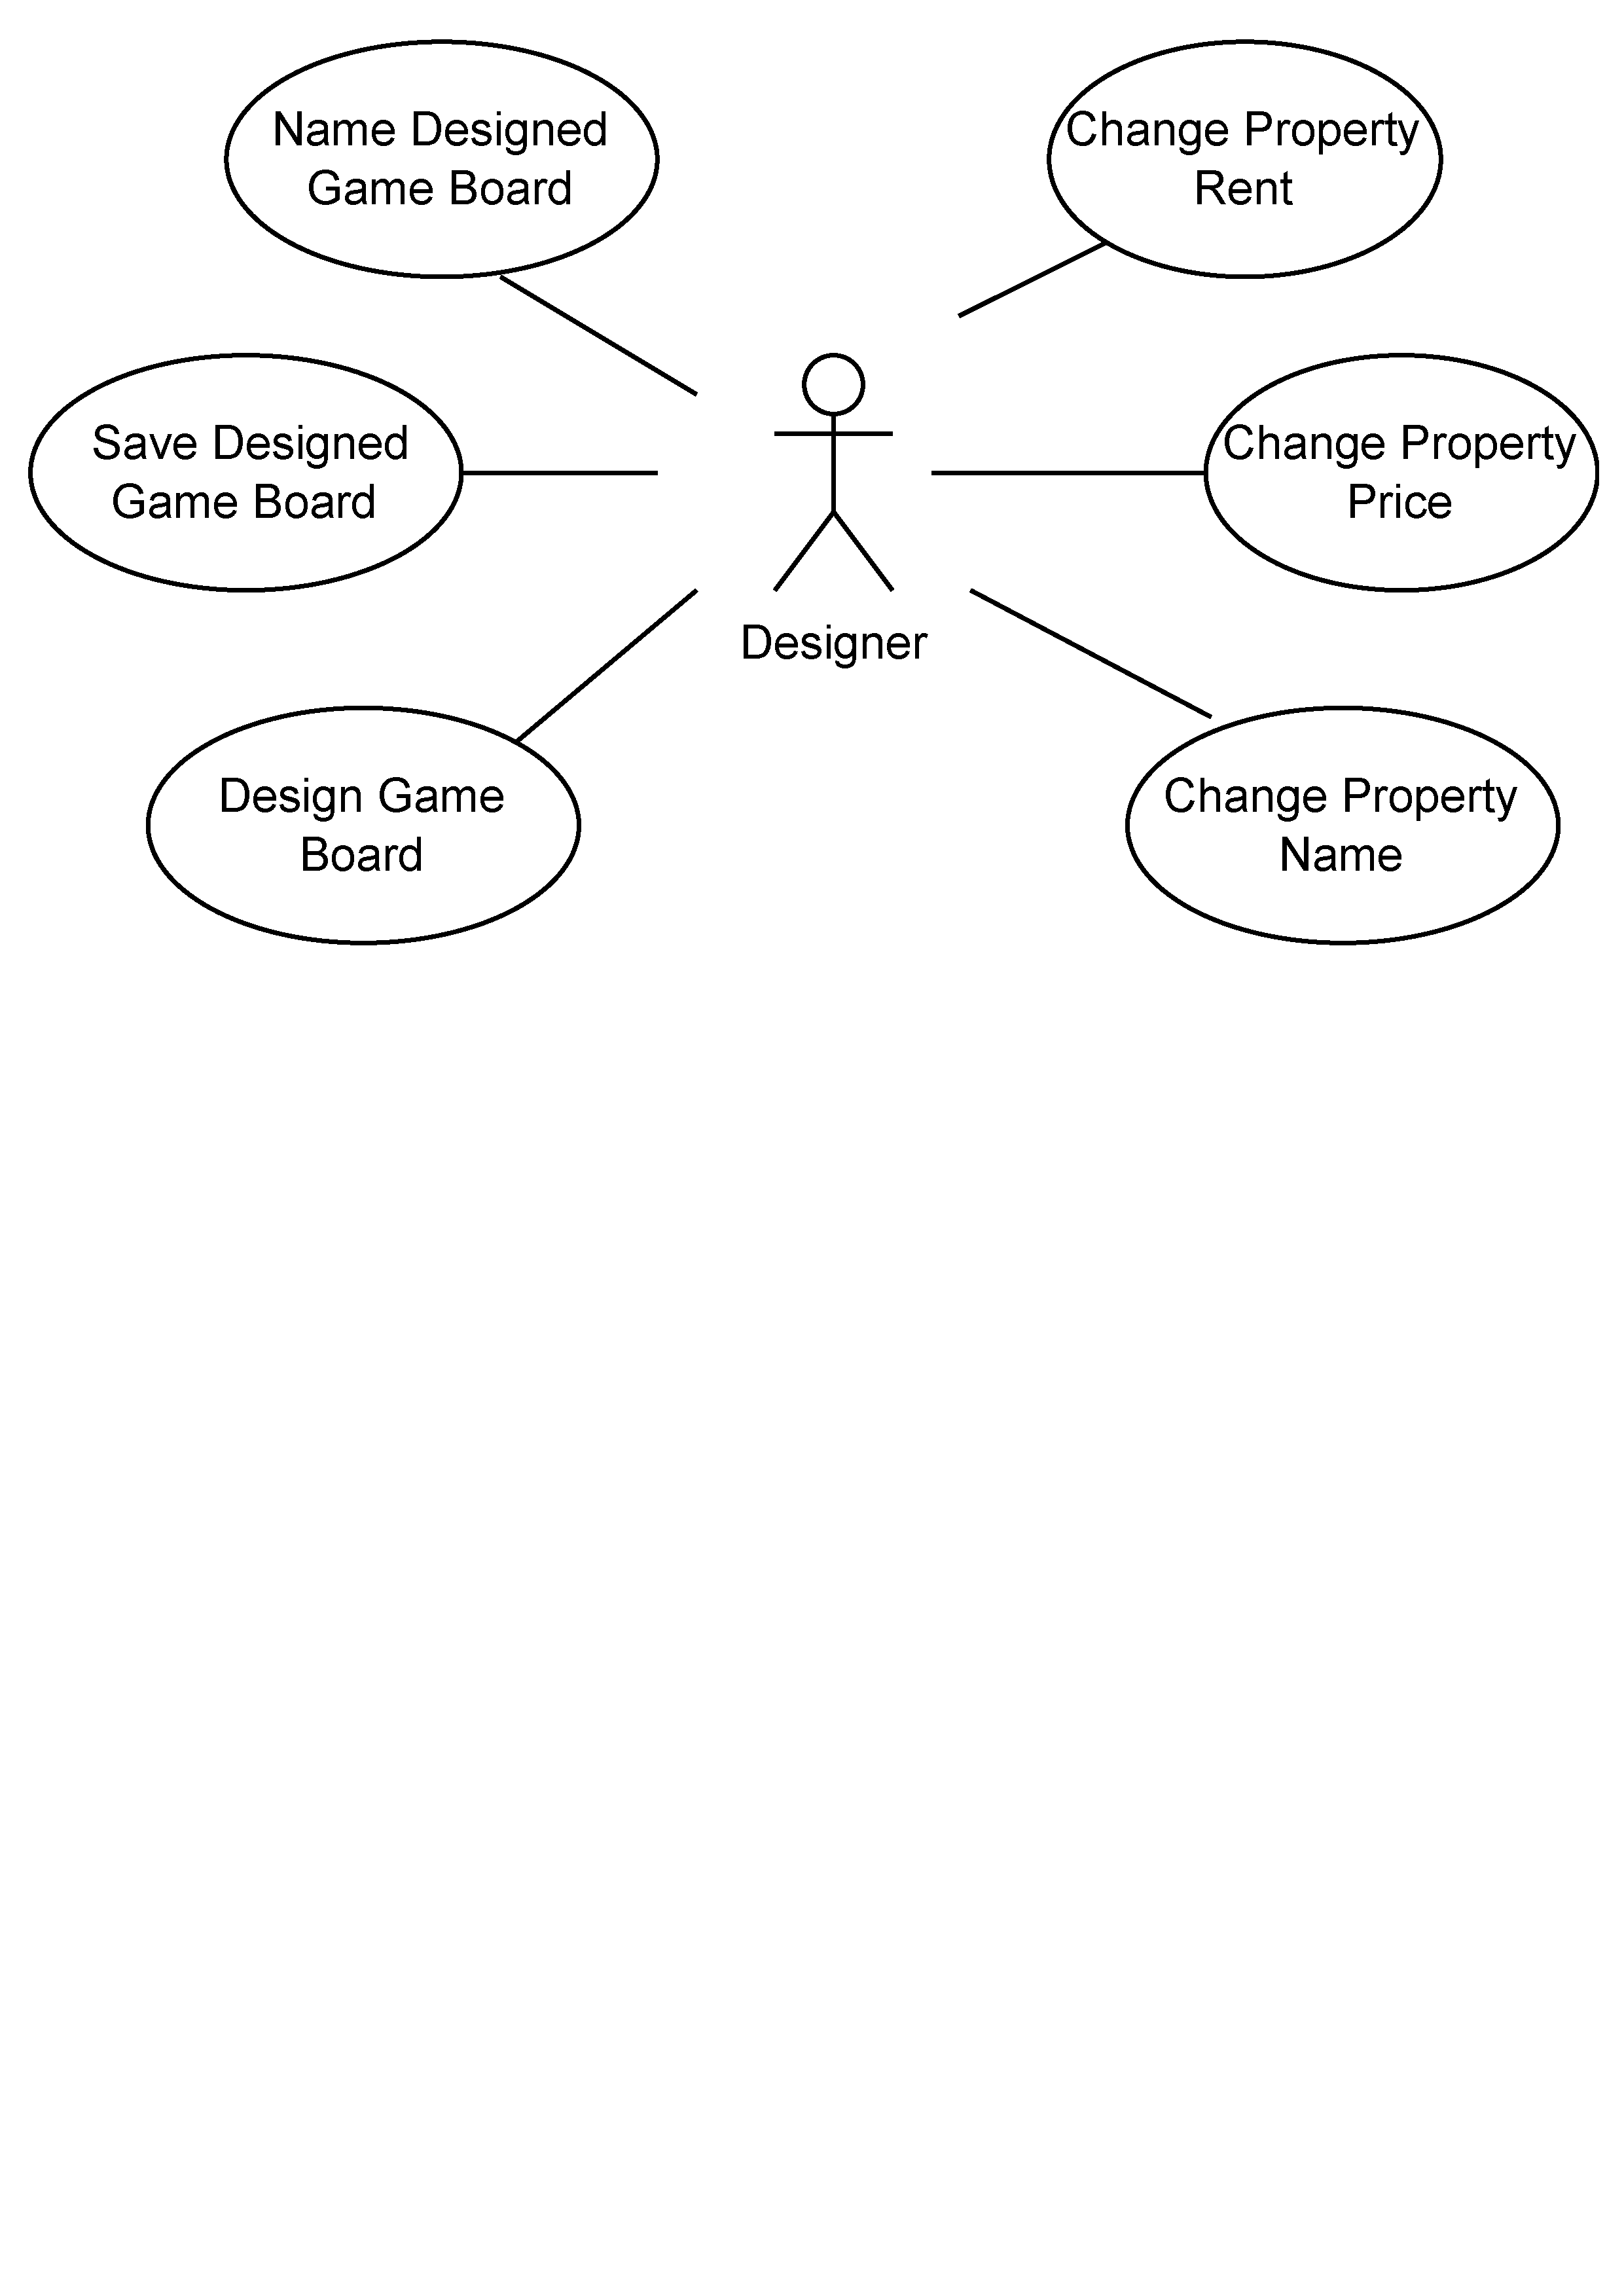
\includegraphics[width=0.6\textwidth]{crop_DesignerUseCases.drawio.pdf}
    \caption{Game Board Designer Use Cases}
\end{figure}

\subsection{User Story 1}

\paragraph{Definition} When starting a new game, a player can opt to start a new game immediately on a default classical 
game board without further need of configuration, or to select a saved custom game board from a file to load before starting the game.
\paragraph{Non-functional Requirements} The navigation flow and the user interface for starting a new game should be intuitive; the processing time of 
loading a default or a saved game board should be less than 1 second.

\subsection{User Story 2}
\paragraph{Definition} At the beginning of the game, the system shall prompt the user to choose to name or to assign a random name to each of the player.
Since players' tokens are represented by the initial letter of their names, the system shall assign different colors to players, and the user will be notified of the color assignment.
In that case, it is unnecessary to forbid players from using the same name as players can always be distinguished by the color of their tokens.
\paragraph{Non-functional Requirements} The system shall ensure that the naming procedure shall not lead to any faults or exceptions.

\subsection{User Story 3}
\paragraph{Definition} When it comes to a player's turn, the player can choose to request the information of a specific player or all players 
about other players' cash, properties, and status in the game.
\paragraph{Non-functional Requirements} The system shall ensure that the information of the players is up to date and displayed in a clear and readable way.

\subsection{User Story 4} 
\paragraph{Definition} A player can always request to print the game board at any time during her turn. After important operations,
the system shall automatically print the game board. Players' tokens shall be displayed on the position they are currently on.
For normal players, their tokens shall be displayed as the capital initial letter between a pair of square brackets, e.g., [A]. 
For players in jail, their tokens shall be displayed as the capital initial letter between a pair of angled brackets, e.g., >A<.
Bankrupted players' tokens shall not be displayed on the game board.
The background color of properties bought by a player shall be set to the color assigned to the player to indicate the ownership.
Apart from the status of the game shown on the game board, the system shall also prompt the current round number and the name of the player whose turn it is at the beginning of the game board.
\paragraph{Non-functional Requirements} The system shall ensure that the game board 
and other information regarding the status of the game is printed in a clear and readable way, and the printing procedure shall not lead to any faults or exceptions.

\subsection{User Story 5}
\paragraph{Definition} When it comes to a player's turn, the player can choose to request the next player after her turn.
\paragraph{Non-functional Requirements} The system shall ensure that the next player's name is correctly identified and displayed with the assigned color.

\subsection{User Story 6}
\paragraph{Definition} When it comes to a player's turn, the player can choose to save the game in progress or a finished game into a file
named by the player.  The game save file shall include all necessary information to reconstruct the game instance for further playing.
\paragraph{Non-functional Requirements} The system shall ensure that the procedure of generating a game save file shall not lead to any faults or exceptions;
the game save file shall be portable to be loaded on any platform that can run the CMG system; the size of the game save file shall be less than 1 MB.

\subsection{User Story 7} 
\paragraph{Definition} The user can choose to load a game save file to reconstruct the game instance to continue playing the game.
The system shall provide a list of game save files for the user to choose from by entering the index of the file.
The status of the game shall be identical to the status when the game was saved.
\paragraph{Non-functional Requirements} The system shall ensure that the procedure of loading a game save file shall not lead to any faults or exceptions;
the processing time of loading a game save file shall be less than 1 second.

\subsection{User Story 8}
\paragraph{Definition} At the main page of the CMG system, the user can choose to design a game board immediately on a default game board without further need of configuration, or to load a saved game board from a file to edit.
The system shall accept the designer's option of modifying a normal property on the game board, and
reject the designer's option of modifying a special property (GO, Income Tax, Chance, Jail Visiting, Go to Jail, Free Parking).
After the designer enters the position of the property to be modified, the system shall print the current information of the property and prompt the designer to select one of 
the following attributes to update: the name of the property, the price of the property, and the rent of the property.
The system shall check the validity of the input of the designer, and update the property information accordingly.
If the user input violates the constraints, the system shall prompt the designer to re-enter the information.
\paragraph{Non-functional Requirements} 
Game board designer shall be able to adapt all functions in the design procedures after 10 minutes of experiencing.
After that, the average number of operational errors designers make shall be less than 1 per 10 minutes.

\subsection{User Story 9}
\paragraph{Definition} The game board designer can select a default game board or a saved game board to load for further editing.
The system shall provide a list of game board files for the designer to choose from by entering the index of the file.
\paragraph{Non-functional Requirements} The system shall ensure that the procedure of loading a game board file shall not lead to any faults or exceptions;
the processing time of loading a game board file shall be less than 1 second.

\subsection{User Story 10}
\paragraph{Definition} The game board designer can choose to save the game board into a file named by the designer after each modification of a property.
The game board file shall include all necessary information to reconstruct the game board for further playing.
\paragraph{Non-functional Requirements} The system shall ensure that the procedure of generating a game board file shall not lead to any faults or exceptions;
the game board file shall be portable to be loaded on any platform that can run the CMG system; the size of the game board file shall be less than 1 MB.

\section{System Architecture}

CMG is supposed to be implement in MVC architecture pattern. Classes defined the game (the gaming procedures), players, properties, and the effects of properties
will be in the model part. Classes defined the view of the game board, the user panel for users' input and selections of operations, and the data structures (Brick and Box) which will assist the print of the game board and game board design procedures, will be in the view package.
The classes defined the procedures of intensive file operations and the initialization of the entire CMG system, the gaming procedures, and the game board design procedures will be in the controller package.

However, for the ease of agile programming, the system will be implemented in a more flexible way. For example, the output routines will also occur in the methods within the controller and model package. In contrast, the 
classes and relevant methods in view are expected to be only responsible for the input and output. Also, methods in the packages will also invoke instances of other packages to perform the operations,
rather than only controller invoking model and view.


\section{System Requirements Specification}



% Table for FR-001
% Set the width for the text in the columns
\newcolumntype{P}[1]{>{\raggedright\arraybackslash}p{#1}}

\subsection{User Story 1}

% Table for FR-001
\begin{table}[ht]
    \centering
    \caption{Functional Requirement FR1.1}
    \begin{tabular}{@{}P{3cm}P{12cm}@{}}
        \toprule
        \textbf{Requirement ID} & FR-001 \\ \midrule
        \textbf{Description} & When the player opts to start a new game, the system shall provide an option to initiate the game using a default classical game board. \\ \midrule
        \textbf{Precondition} & The player is on the main menu or game start screen. \\ \midrule
        \textbf{Postcondition} & A new game is started immediately using the default classical game board without requiring any additional configuration from the player. \\ \bottomrule
    \end{tabular}
\end{table}

% Table for FR-002
\begin{table}[ht]
    \centering
    \caption{Functional Requirement FR-1.2}
    \begin{tabular}{@{}P{3cm}P{12cm}@{}}
        \toprule
        \textbf{Requirement ID} & FR-002 \\ \midrule
        \textbf{Description} & The system shall present the player with an option to load a saved custom game board from a file before starting the new game. \\ \midrule
        \textbf{Precondition} & The player chooses the option to start a new game and selects "Load Custom Board." \\ \midrule
        \textbf{Postcondition} & The system allows the player to browse and select a saved game board file. Upon selection, the game shall load the custom game board and then allow the player to start the game. \\ \bottomrule
    \end{tabular}
\end{table}

% Table for FR-003
\begin{table}[ht]
    \centering
    \caption{Functional Requirement FR-1.3}
    \begin{tabular}{@{}P{3cm}P{12cm}@{}}
        \toprule
        \textbf{Requirement ID} & FR-003 \\ \midrule
        \textbf{Description} & When the player opts to load a saved custom game board, the system shall provide a file selection dialog that displays all compatible game board files stored on the player's device. \\ \midrule
        \textbf{Precondition} & The player has selected "Load Custom Board" and is presented with the file selection dialog. \\ \midrule
        \textbf{Postcondition} & The player can navigate directories and select a custom game board file. If a valid file is selected, it is loaded; if an invalid file is selected, an error message is displayed indicating the error. \\ \bottomrule
    \end{tabular}
\end{table}


\begin{table}[ht]
    \centering
    \caption{Functional Requirement FR-1.4}
    \begin{tabular}{@{}P{3cm}P{12cm}@{}}
        \toprule
        \textbf{Requirement ID} & FR-005 \\ \midrule
        \textbf{Description} & Upon successfully loading a custom game board, the system shall display a confirmation message indicating that the custom game board has been loaded successfully and the game is ready to start. \\ \midrule
        \textbf{Precondition} & The custom game board has been correctly loaded into the game. \\ \midrule
        \textbf{Postcondition} & The confirmation message prompts the player to start the game, and the game begins using the loaded custom game board. \\ \bottomrule
    \end{tabular}
\end{table}

\clearpage

\subsection{User Story 2}

%Table for FR-2.1
\begin{table}[ht]
    \centering
    \caption{Functional Requirement FR-2.1}
    \begin{tabular}{@{}P{3cm}P{12cm}@{}}
        \toprule
        \textbf{Requirement ID} & FR-2.1 \\ \midrule
        \textbf{Description} & At the beginning of the game, the system shall prompt the user to choose to name or to assign a random name to each of the players. \\ \midrule
        \textbf{Precondition} & The game has initiated but has not yet begun. \\ \midrule
        \textbf{Postcondition} & The user is presented with options for naming players or allowing the system to assign random names. \\ \bottomrule
    \end{tabular}
\end{table}

% Table for FR-2.2
\begin{table}[ht]
    \centering
    \caption{Functional Requirement FR-2.2}
    \begin{tabular}{@{}P{3cm}P{12cm}@{}}
        \toprule
        \textbf{Requirement ID} & FR-2.2 \\ \midrule
        \textbf{Description} & Once the names have been assigned, the system shall assign different colors to each player’s token. \\ \midrule
        \textbf{Precondition} & Player names have been established through user input or random assignment. \\ \midrule
        \textbf{Postcondition} & Each player is assigned a unique color for their token that will be visible during the game. \\ \bottomrule
    \end{tabular}
\end{table}

% Table for FR-2.3
\begin{table}[ht]
    \centering
    \caption{Functional Requirement FR-2.3}
    \begin{tabular}{@{}P{3cm}P{12cm}@{}}
        \toprule
        \textbf{Requirement ID} & FR-2.3 \\ \midrule
        \textbf{Description} & The system shall notify the user of the color assignments for each player after the colors have been assigned. \\ \midrule
        \textbf{Precondition} & Players have been assigned colors to their tokens following name assignment. \\ \midrule
        \textbf{Postcondition} & Users receive a message indicating which colors are assigned to each player’s token. \\ \bottomrule
    \end{tabular}
\end{table}

% Table for FR-2.4
\begin{table}[ht]
    \centering
    \caption{Functional Requirement FR-2.4}
    \begin{tabular}{@{}P{3cm}P{12cm}@{}}
        \toprule
        \textbf{Requirement ID} & FR-2.4 \\ \midrule
        \textbf{Description} & The system shall not forbid players from using the same name, as each player can always be distinguished by the color of their tokens. \\ \midrule
        \textbf{Precondition} & The option to name players is available and accessible to the user. \\ \midrule
        \textbf{Postcondition} & Players are allowed to select identical names; differentiation is maintained through color assignments. \\ \bottomrule
    \end{tabular}
\end{table}

\clearpage
\subsection{User Story 3}

\begin{table}[ht]
    \centering
    \caption{Functional Requirement FR-3.1}
    \begin{tabular}{@{}P{3cm}P{12cm}@{}}
        \toprule
        \textbf{Requirement ID} & FR-2.5 \\ \midrule
        \textbf{Description} & When it is a player’s turn, the player shall be able to request information about a specific player’s cash, properties, and status in the game. \\ \midrule
        \textbf{Precondition} & It is the current player’s turn in the game. \\ \midrule
        \textbf{Postcondition} & The game system retrieves and presents the requested information about the specific player. \\ \bottomrule
    \end{tabular}
\end{table}

\begin{table}[ht]
    \centering
    \caption{Functional Requirement FR-3.2}
    \begin{tabular}{@{}P{3cm}P{12cm}@{}}
        \toprule
        \textbf{Requirement ID} & FR-2.6 \\ \midrule
        \textbf{Description} & In addition to requesting information about a specific player, the system shall allow the player to request information about all players regarding their cash, properties, and status in the game. \\ \midrule
        \textbf{Precondition} & It is the current player’s turn in the game. \\ \midrule
        \textbf{Postcondition} & The game system retrieves and presents the requested information for all players. \\ \bottomrule
    \end{tabular}
\end{table}

\clearpage
\subsection{User Story 4}

% Table for FR-4.1
\begin{table}[ht]
    \centering
    \caption{Functional Requirement FR-4.1}
    \begin{tabular}{@{}P{3cm}P{12cm}@{}}
        \toprule
        \textbf{Requirement ID} & FR-4.1 \\ \midrule
        \textbf{Description} & A player shall be able to request the game board to be printed at any time during her turn. \\ \midrule
        \textbf{Precondition} & The game is in progress, and it is the current player's turn. \\ \midrule
        \textbf{Postcondition} & The game board is printed, showing the current state of the game, including player positions. \\ \bottomrule
    \end{tabular}
\end{table}

% Table for FR-4.2
\begin{table}[ht]
    \centering
    \caption{Functional Requirement FR-4.2}
    \begin{tabular}{@{}P{3cm}P{12cm}@{}}
        \toprule
        \textbf{Requirement ID} & FR-4.2 \\ \midrule
        \textbf{Description} & After important operations in the game, the system shall automatically print the game board. \\ \midrule
        \textbf{Precondition} & A significant event or operation (e.g., a player’s move) occurs during the game. \\ \midrule
        \textbf{Postcondition} & The updated game board is printed to reflect the changes made by the operation. \\ \bottomrule
    \end{tabular}
\end{table}

% Table for FR-4.3
\begin{table}[ht]
    \centering
    \caption{Functional Requirement FR-4.3}
    \begin{tabular}{@{}P{3cm}P{12cm}@{}}
        \toprule
        \textbf{Requirement ID} & FR-4.3 \\ \midrule
        \textbf{Description} & Players' tokens shall be displayed on the position they lands on on the game board. For normal players, their tokens shall be displayed as the capital initial letter between a pair of square brackets, e.g., [A]. For players in jail, their tokens shall be displayed as the capital initial letter between a pair of angled brackets, e.g., >A<. Bankrupted players’ tokens shall not be displayed on the game board. \\ \midrule
        \textbf{Precondition} & The game board is being printed or displayed. \\ \midrule
        \textbf{Postcondition} & The positions of all active players' tokens are correctly represented based on their status. \\ \bottomrule
    \end{tabular}
\end{table}

% Table for FR-4.4
\begin{table}[ht]
    \centering
    \caption{Functional Requirement FR-4.4}
    \begin{tabular}{@{}P{3cm}P{12cm}@{}}
        \toprule
        \textbf{Requirement ID} & FR-4.4 \\ \midrule
        \textbf{Description} & The background color of properties owned by a player shall be set to the color assigned to that player to indicate ownership. \\ \midrule
        \textbf{Precondition} & Properties have been bought and ownership has been assigned. \\ \midrule
        \textbf{Postcondition} & The game board visually reflects the ownership of properties through color coding. \\ \bottomrule
    \end{tabular}
\end{table}

% Table for FR-4.5
\begin{table}[ht]
    \centering
    \caption{Functional Requirement FR-4.5}
    \begin{tabular}{@{}P{3cm}P{12cm}@{}}
        \toprule
        \textbf{Requirement ID} & FR-4.5 \\ \midrule
        \textbf{Description} & The system shall prompt the current round number and the name of the player whose turn it is at the beginning of the game board display. \\ \midrule
        \textbf{Precondition} & The game is beginning or transitioning to a new round. \\ \midrule
        \textbf{Postcondition} & The game board display includes the current round number and the active player's name prominently. \\ \bottomrule
    \end{tabular}
\end{table}

\clearpage
\subsection{User Story 5}

% Table for FR-5.1
\begin{table}[ht]
    \centering
    \caption{Functional Requirement FR-5.1}
    \begin{tabular}{@{}P{3cm}P{12cm}@{}}
        \toprule
        \textbf{Requirement ID} & FR-5.1 \\ \midrule
        \textbf{Description} & When it is a player’s turn, the player shall be able to request information about the next player after her turn. \\ \midrule
        \textbf{Precondition} & It is the current player’s turn in the game. \\ \midrule
        \textbf{Postcondition} & The game system retrieves and presents information about the next player in turn order. \\ \bottomrule
    \end{tabular}
\end{table}

\clearpage
\subsection{User Story 6}
% Table for FR-6.1
\begin{table}[ht]
    \centering
    \caption{Functional Requirement FR-6.1}
    \begin{tabular}{@{}P{3cm}P{12cm}@{}}
        \toprule
        \textbf{Requirement ID} & FR-6.1 \\ \midrule
        \textbf{Description} & When it is a player’s turn, the player shall be able to save the game in progress or a finished game into a file named by the player. \\ \midrule
        \textbf{Precondition} & The game is currently in progress, or a game has been finished. \\ \midrule
        \textbf{Postcondition} & The game state is saved to a file, allowing for future playback and reconstruction of the game instance. \\ \bottomrule
    \end{tabular}
\end{table}

% Table for FR-6.1
\begin{table}[ht]
    \centering
    \caption{Functional Requirement FR-6.2}
    \begin{tabular}{@{}P{3cm}P{12cm}@{}}
        \toprule
        \textbf{Requirement ID} & FR-6.1 \\ \midrule
        \textbf{Description} & The game save file shall contain all necessary information of the game, players, and properties for complete reinitialization when loading. \\ \midrule
        \textbf{Precondition} & The game is currently in progress, or a game has been finished. \\ \midrule
        \textbf{Postcondition} & The game state is saved to a file, allowing for future playback and reconstruction of the game instance. \\ \bottomrule
    \end{tabular}
\end{table}

\clearpage
\subsection{User Story 7}

% Table for FR-7.1
\begin{table}[ht]
    \centering
    \caption{Functional Requirement FR-7.1}
    \begin{tabular}{@{}P{3cm}P{12cm}@{}}
        \toprule
        \textbf{Requirement ID} & FR-7.1 \\ \midrule
        \textbf{Description} & The user shall be able to choose to load a game save file to reconstruct the game instance and continue playing. \\ \midrule
        \textbf{Precondition} & Available game save files exist that can be loaded. \\ \midrule
        \textbf{Postcondition} & The game instance is successfully reconstructed from the selected save file. \\ \bottomrule
    \end{tabular}
\end{table}

% Table for FR-7.2
\begin{table}[ht]
    \centering
    \caption{Functional Requirement FR-7.2}
    \begin{tabular}{@{}P{3cm}P{12cm}@{}}
        \toprule
        \textbf{Requirement ID} & FR-7.2 \\ \midrule
        \textbf{Description} & The system shall provide a list of game save files for the user to choose from by entering the index of the file. \\ \midrule
        \textbf{Precondition} & The user is in the process of loading a game. \\ \midrule
        \textbf{Postcondition} & The user has selected a game save file from the list. \\ \bottomrule
    \end{tabular}
\end{table}

% Table for FR-7.3
\begin{table}[ht]
    \centering
    \caption{Functional Requirement FR-7.3}
    \begin{tabular}{@{}P{3cm}P{12cm}@{}}
        \toprule
        \textbf{Requirement ID} & FR-7.3 \\ \midrule
        \textbf{Description} & The status of the game shall be identical to the status when the game was saved. \\ \midrule
        \textbf{Precondition} & A game save file has been successfully loaded. \\ \midrule
        \textbf{Postcondition} & The game status matches the saved state at the time of the save. \\ \bottomrule
    \end{tabular}
\end{table}

\clearpage
\subsection{User Story 8}

% Table for FR-8.1
\begin{table}[ht]
    \centering
    \caption{Functional Requirement FR-8.1}
    \begin{tabular}{@{}P{3cm}P{12cm}@{}}
        \toprule
        \textbf{Requirement ID} & FR-8.1 \\ \midrule
        \textbf{Description} & At the main page of the CMG system, the user can choose to design a game board immediately on a default game board without further need of configuration, or to load a saved game board from a file to edit. \\ \midrule
        \textbf{Precondition} & The user is on the main page of the CMG system. \\ \midrule
        \textbf{Postcondition} & The user has selected an option to either design or load a game board. \\ \bottomrule
    \end{tabular}
\end{table}

% Table for FR-8.2
\begin{table}[ht]
    \centering
    \caption{Functional Requirement FR-8.2}
    \begin{tabular}{@{}P{3cm}P{12cm}@{}}
        \toprule
        \textbf{Requirement ID} & FR-8.2 \\ \midrule
        \textbf{Description} & The system shall accept the designer’s option of modifying a normal property on the game board and reject the designer’s option of modifying a special property (GO, Income Tax, Chance, Jail Visiting, Go to Jail, Free Parking). \\ \midrule
        \textbf{Precondition} & The designer is attempting to modify a property on the game board. \\ \midrule
        \textbf{Postcondition} & The system either allows or denies the modification based on the property type. \\ \bottomrule
    \end{tabular}
\end{table}

% Table for FR-8.3
\begin{table}[ht]
    \centering
    \caption{Functional Requirement FR-8.3}
    \begin{tabular}{@{}P{3cm}P{12cm}@{}}
        \toprule
        \textbf{Requirement ID} & FR-8.3 \\ \midrule
        \textbf{Description} & After the designer enters the position of the property to be modified, the system shall print the current information of the property and prompt the designer to select one of the following attributes to update: the name of the property, the price of the property, and the rent of the property. \\ \midrule
        \textbf{Precondition} & The designer has entered a valid property position. \\ \midrule
        \textbf{Postcondition} & The system displays the current property information and prompts for attribute selection. \\ \bottomrule
    \end{tabular}
\end{table}

% Table for FR-8.4
\begin{table}[ht]
    \centering
    \caption{Functional Requirement FR-8.4}
    \begin{tabular}{@{}P{3cm}P{12cm}@{}}
        \toprule
        \textbf{Requirement ID} & FR-8.4 \\ \midrule
        \textbf{Description} & The system shall check the validity of the input of the designer and update the property information accordingly. If the user input violates the constraints, the system shall prompt the designer to re-enter the information. \\ \midrule
        \textbf{Precondition} & The designer has selected an attribute to update and entered the new value. \\ \midrule
        \textbf{Postcondition} & The property information is updated if valid; otherwise, the designer is prompted to re-enter the information. \\ \bottomrule
    \end{tabular}
\end{table}

\clearpage
\subsection{User Story 9}

% Table for FR-9.1
\begin{table}[ht]
    \centering
    \caption{Functional Requirement FR-9.1}
    \begin{tabular}{@{}P{3cm}P{12cm}@{}}
        \toprule
        \textbf{Requirement ID} & FR-9.1 \\ \midrule
        \textbf{Description} & The game board designer can select a default game board or a saved game board to load for further editing. \\ \midrule
        \textbf{Precondition} & The designer is on the game board selection interface. \\ \midrule
        \textbf{Postcondition} & The designer has selected either a default or a saved game board for editing. \\ \bottomrule
    \end{tabular}
\end{table}

% Table for FR-9.2
\begin{table}[ht]
    \centering
    \caption{Functional Requirement FR-9.2}
    \begin{tabular}{@{}P{3cm}P{12cm}@{}}
        \toprule
        \textbf{Requirement ID} & FR-9.2 \\ \midrule
        \textbf{Description} & The system shall provide a list of game board files for the designer to choose from by entering the index of the file. \\ \midrule
        \textbf{Precondition} & The designer has selected the option to load a saved game board. \\ \midrule
        \textbf{Postcondition} & The system displays a list of available game board files along with their indices. \\ \bottomrule
    \end{tabular}
\end{table}

\clearpage
\subsection{User Story 10}

% Table for FR-10.1
\begin{table}[ht]
    \centering
    \caption{Functional Requirement FR-10.1}
    \begin{tabular}{@{}P{3cm}P{12cm}@{}}
        \toprule
        \textbf{Requirement ID} & FR-10.1 \\ \midrule
        \textbf{Description} & The game board designer can choose to save the game board into a file named by the designer after each modification of a property. \\ \midrule
        \textbf{Precondition} & The designer has made modifications to the game board properties. \\ \midrule
        \textbf{Postcondition} & The game board is saved into a file with the chosen name. \\ \bottomrule
    \end{tabular}
\end{table}

% Table for FR-10.2
\begin{table}[ht]
    \centering
    \caption{Functional Requirement FR-10.2}
    \begin{tabular}{@{}P{3cm}P{12cm}@{}}
        \toprule
        \textbf{Requirement ID} & FR-10.2 \\ \midrule
        \textbf{Description} & The game board file shall include all necessary information to reconstruct the game board for further playing. \\ \midrule
        \textbf{Precondition} & The game board has been modified and is ready to be saved. \\ \midrule
        \textbf{Postcondition} & The saved file contains all required details to accurately recreate the game board state. \\ \bottomrule
    \end{tabular}
\end{table}

\subsection{Other Essential Functional Requirements}

% Table for FR-11.1
\begin{table}[ht]
    \centering
    \caption{Functional Requirement FR-11.1}
    \begin{tabular}{@{}P{3cm}P{12cm}@{}}
        \toprule
        \textbf{Requirement ID} & FR-11.1 \\ \midrule
        \textbf{Description} & The system shall claim the game over when only one player who is not bankrupted is left, or the total number of rounds reaches 100. \\ \midrule
        \textbf{Precondition} & The game is in progress, and the conditions for game over are met. \\ \midrule
        \textbf{Postcondition} & The game is declared over, and the final status of the game is displayed. \\ \bottomrule
    \end{tabular}
\end{table}

% Table for FR-11.2
\begin{table}[ht]
    \centering
    \caption{Functional Requirement FR-11.2}
    \begin{tabular}{@{}P{3cm}P{12cm}@{}}
        \toprule
        \textbf{Requirement ID} & FR-11.2 \\ \midrule
        \textbf{Description} & The system shall update the player's status to "in jail" when the player lands on the "Go to Jail" property. \\ \midrule
        \textbf{Precondition} & The player lands on the "Go to Jail" property. \\ \midrule
        \textbf{Postcondition} & The player's status is updated to "in jail," and the player is moved to the Jail property. \\ \bottomrule
    \end{tabular}
\end{table}

% Table for FR-11.3
\begin{table}[ht]
    \centering
    \caption{Functional Requirement FR-11.3}
    \begin{tabular}{@{}P{3cm}P{12cm}@{}}
        \toprule
        \textbf{Requirement ID} & FR-11.3 \\ \midrule
        \textbf{Description} & The system shall update the player's status to "bankrupt" when the player's cash is less than 0 after paying rent or penalty. \\ \midrule
        \textbf{Precondition} & The player's cash is less than 0 after a transaction. \\ \midrule
        \textbf{Postcondition} & The player's status is updated to "bankrupt," and the player is removed from the ongoing players. \\ \bottomrule
    \end{tabular}
\end{table}

% Table for FR-11.4
\begin{table}[ht]
    \centering
    \caption{Functional Requirement FR-11.4}
    \begin{tabular}{@{}P{3cm}P{12cm}@{}}
        \toprule
        \textbf{Requirement ID} & FR-11.4 \\ \midrule
        \textbf{Description} & The system shall allow a player to buy a property if the property is not owned by any player and the player has enough cash to buy it. \\ \midrule
        \textbf{Precondition} & The player lands on an unowned property and has sufficient cash. \\ \midrule
        \textbf{Postcondition} & The property is bought by the player, and the player's cash is reduced by the property's price. \\ \bottomrule
    \end{tabular}
\end{table}

% Table for FR-11.5
\begin{table}[ht]
    \centering
    \caption{Functional Requirement FR-11.5}
    \begin{tabular}{@{}P{3cm}P{12cm}@{}}
        \toprule
        \textbf{Requirement ID} & FR-11.5 \\ \midrule
        \textbf{Description} & The system shall allow a player to collect rent from another player who lands on their property. \\ \midrule
        \textbf{Precondition} & Another player lands on a property owned by the player. \\ \midrule
        \textbf{Postcondition} & The owner player receives rent, and the landing player's cash is reduced by the rent amount. \\ \bottomrule
    \end{tabular}
\end{table}

% Table for FR-11.6
\begin{table}[ht]
    \centering
    \caption{Functional Requirement FR-11.6}
    \begin{tabular}{@{}P{3cm}P{12cm}@{}}
        \toprule
        \textbf{Requirement ID} & FR-11.6 \\ \midrule
        \textbf{Description} & The system shall give a salary of HKD1500 to every player each time they pass through the GO property. \\ \midrule
        \textbf{Precondition} & The player passes through the GO property. \\ \midrule
        \textbf{Postcondition} & The player's cash is increased by HKD1500. \\ \bottomrule
    \end{tabular}
\end{table}

% Table for FR-11.7
\begin{table}[ht]
    \centering
    \caption{Functional Requirement FR-11.7}
    \begin{tabular}{@{}P{3cm}P{12cm}@{}}
        \toprule
        \textbf{Requirement ID} & FR-11.7 \\ \midrule
        \textbf{Description} & The system shall charge the player 10\% of her money (rounded down to a multiple of 10) when the player lands on the Income Tax property. \\ \midrule
        \textbf{Precondition} & The player lands on the Income Tax property. \\ \midrule
        \textbf{Postcondition} & The player's cash is reduced by 10\% (rounded down to a multiple of 10). \\ \bottomrule
    \end{tabular}
\end{table}

% Table for FR-11.8
\begin{table}[ht]
    \centering
    \caption{Functional Requirement FR-11.8}
    \begin{tabular}{@{}P{3cm}P{12cm}@{}}
        \toprule
        \textbf{Requirement ID} & FR-11.8 \\ \midrule
        \textbf{Description} & The system shall trigger a random change on the player's money when the player lands on the Chance property. The change is a multiple of 10 from -200 to 300. \\ \midrule
        \textbf{Precondition} & The player lands on the Chance property. \\ \midrule
        \textbf{Postcondition} & The player's cash is adjusted by a random amount between -200 and 300, in multiples of 10. \\ \bottomrule
    \end{tabular}
\end{table}

% Table for FR-11.9
\begin{table}[ht]
    \centering
    \caption{Functional Requirement FR-11.9}
    \begin{tabular}{@{}P{3cm}P{12cm}@{}}
        \toprule
        \textbf{Requirement ID} & FR-11.9 \\ \midrule
        \textbf{Description} & The system shall not affect the player's status when the player lands on the Jail Visiting property. \\ \midrule
        \textbf{Precondition} & The player lands on the Jail Visiting property. \\ \midrule
        \textbf{Postcondition} & The player's status remains unchanged. \\ \bottomrule
    \end{tabular}
\end{table}

% Table for FR-11.10
\begin{table}[ht]
    \centering
    \caption{Functional Requirement FR-11.10}
    \begin{tabular}{@{}P{3cm}P{12cm}@{}}
        \toprule
        \textbf{Requirement ID} & FR-11.10 \\ \midrule
        \textbf{Description} & The system shall send the player to the Jail property when the player lands on the Go to Jail property. \\ \midrule
        \textbf{Precondition} & The player lands on the Go to Jail property. \\ \midrule
        \textbf{Postcondition} & The player is moved to the Jail property and their status is updated to "in jail." \\ \bottomrule
    \end{tabular}
\end{table}

% Table for FR-11.11
\begin{table}[ht]
    \centering
    \caption{Functional Requirement FR-11.11}
    \begin{tabular}{@{}P{3cm}P{12cm}@{}}
        \toprule
        \textbf{Requirement ID} & FR-11.11 \\ \midrule
        \textbf{Description} & The system shall allow a player in jail to exit by rolling identical numbers on both dice (doubles) within her next three turns, or by paying a fee of HKD 150 before rolling the dice on her subsequent two turns. If the player fails to roll doubles within the three turns, she must pay HKD 150 to exit jail. \\ \midrule
        \textbf{Precondition} & The player is in jail. \\ \midrule
        \textbf{Postcondition} & The player exits jail either by rolling doubles or paying the fee, and moves the number of spaces indicated by her subsequent dice roll. \\ \bottomrule
    \end{tabular}
\end{table}

% Table for FR-11.12
\begin{table}[ht]
    \centering
    \caption{Functional Requirement FR-11.12}
    \begin{tabular}{@{}P{3cm}P{12cm}@{}}
        \toprule
        \textbf{Requirement ID} & FR-11.12 \\ \midrule
        \textbf{Description} & The system shall not affect the player's status when the player lands on the Free Parking property. \\ \midrule
        \textbf{Precondition} & The player lands on the Free Parking property. \\ \midrule
        \textbf{Postcondition} & The player's status remains unchanged. \\ \bottomrule
    \end{tabular}
\end{table}

\end{document}